
\documentclass{beamer}
\usecolortheme{dove}
\setbeamertemplate{navigation symbols}{}
\usepackage{amsmath,amssymb,amsfonts,amsthm, multicol, subfigure, color}
\usepackage{bm}
\usepackage{graphicx}
\usepackage{tabularx}
\usepackage{booktabs}
\usepackage{hyperref}
\usepackage{pdfpages}
\usepackage{xcolor}
\definecolor{seagreen}{RGB}{46, 139, 87}
\def\independenT#1#2{\mathrel{\rlap{$#1#2$}\mkern2mu{#1#2}}}
\newcommand\indep{\protect\mathpalette{\protect\independenT}{\perp}}
\def\log{\text{log}}
\newcommand\logit{\text{logit}}
\newcommand\iid{\stackrel{\text{iid}}{\sim}}
\newcommand\E{\text{E}}
\newcommand\V{\text{V}}
\renewcommand\P{\text{P}}
\newcommand{\Cov}{\text{Cov}}
\newcommand{\Cor}{\text{Cor}}
\newcommand\doop{\texttt{do}}
\usepackage{stackrel}
\usepackage{tikz}
\usetikzlibrary{arrows,shapes.arrows,positioning,shapes,patterns,calc}
\newcommand\slideref[1]{\vskip .1cm \tiny \textcolor{gray}{{#1}}}
\newcommand\red[1]{\color{red}#1}
\newcommand\blue[1]{\color{blue}#1}
\newcommand\gray[1]{\color{gray}#1}
\newcommand\seagreen[1]{\color{seagreen}#1}
\newcommand\purple[1]{\color{purple}#1}
\newcommand\orange[1]{\color{orange}#1}
\newcommand\black[1]{\color{black}#1}
\newcommand\white[1]{\color{white}#1}
\newcommand\teal[1]{\color{teal}#1}
\newcommand\magenta[1]{\color{magenta}#1}
\newcommand\Fuchsia[1]{\color{Fuchsia}#1}
\newcommand\BlueGreen[1]{\color{BlueGreen}#1}
\newcommand\bblue[1]{\textcolor{blue}{\textbf{#1}}}
\newcommand\bred[1]{\textcolor{red}{\textbf{#1}}}
\newcommand\bgray[1]{\textcolor{gray}{\textbf{#1}}}
\newcommand\bgreen[1]{\textcolor{seagreen}{\textbf{#1}}}
\newcommand\bref[2]{\href{#1}{\color{blue}{#2}}}
\colorlet{lightgray}{gray!40}
\pgfdeclarelayer{bg}    % declare background layer for tikz
\pgfsetlayers{bg,main} % order layers for tikz
\newcommand\mycite[1]{\begin{scriptsize}\textcolor{darkgray}{(#1)}\end{scriptsize}}
\newcommand{\tcframe}{\frame{
%\small{
\only<1|handout:0>{\tableofcontents}
\only<2|handout:1>{\tableofcontents[currentsubsection]}}
%}
}

\usepackage[round]{natbib}
\bibliographystyle{humannat-mod}
\setbeamertemplate{enumerate items}[default]
\usepackage{mathtools}
\usepackage{ulem}

% Need to add examples

\newcommand{\goalsframe}{\begin{frame}{Learning goals for today}
At the end of class, you will be able to:
\begin{enumerate}
\item Recognize the promises and pitfalls of four methods to study the effects of treatments that turn on once
\begin{enumerate}
\item Difference in difference (DID)
\item Interrupted time series (ITS)
\item Regression discontinuity (RD)
\item Synthetic control (SC)
\end{enumerate}
\end{enumerate} \vskip .2in
\end{frame}}

\title{22. Treatments that turn on once\vskip .1in\begin{small}Difference in difference\\Interrupted time series\\Regression discontinuity\\Synthetic control\\{}\end{small}}
\author{Ian Lundberg\\Cornell Info 6751: Causal Inference in Observational Settings\\Fall 2022}
\date{8 Nov 2022}

\begin{document}

\maketitle

\goalsframe

\begin{frame}

Economic theory: A higher minimum wage reduces employment \vskip .2in \pause
Data
\begin{itemize}
\item Apr 1 1991: Federal minimum wage rises to \$4.25
\item Apr 1 1992: New Jersey minimum wage rises to \$5.05
\end{itemize} \vskip .2in \pause
\bgray{Theoretical Estimand}: Effect of the law on employment in NJ \pause
$$\underbrace{Y_\text{NJ,After}^1}_\text{Observed}\quad  - \underbrace{Y_\text{NJ,After}^0}_\text{Counterfactual}$$
where $Y$ is employment, \\ \pause
superscript $A = 1$ is \$5.05 minimum wage, and\\ pause
superscript $A = 0$ is \$4.25 minimum wage

\end{frame}

\begin{frame}
\begin{tikzpicture}[x = \textwidth, y = \textheight]
\node at (.5,.5) {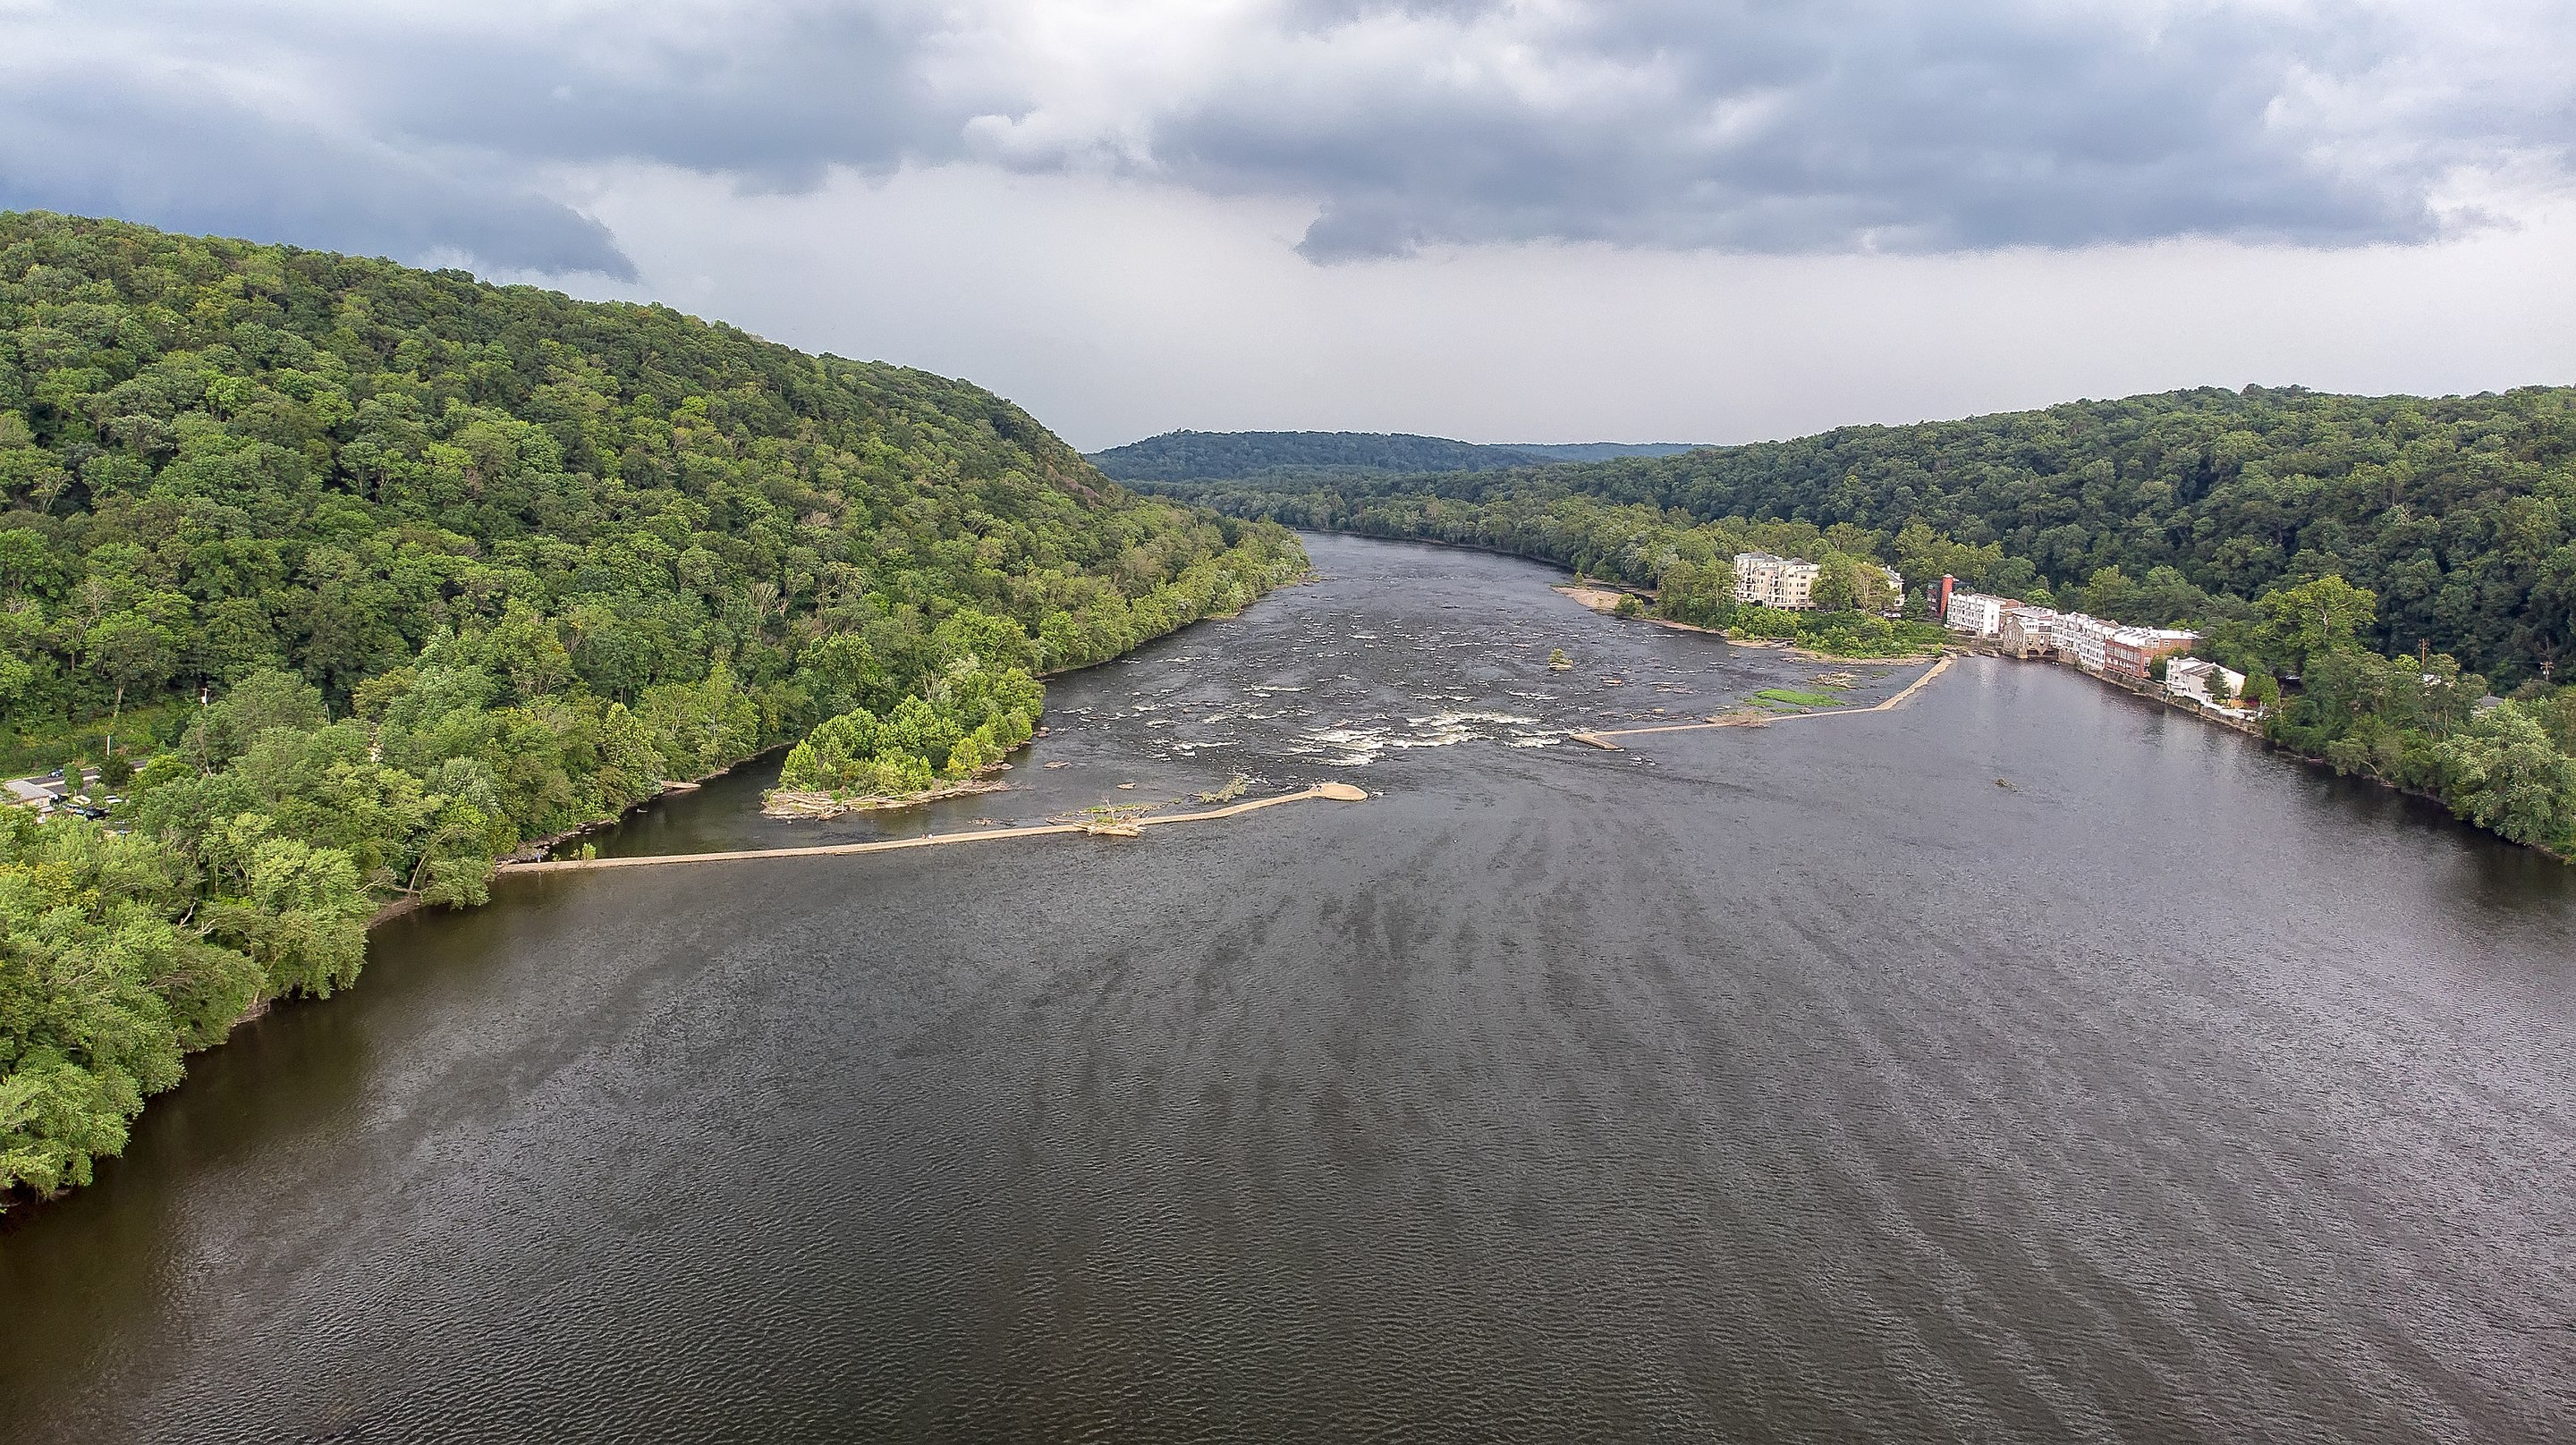
\includegraphics[width = \textwidth]{figures/Delaware_River}};
\node[anchor = south east, font = \tiny, align = center] at (1,0) {Photo by James Loesch - https://www.flickr.com/photos/jal33/49113053632/\\CC BY 2.0, https://commons.wikimedia.org/w/index.php?curid=87207834}; \pause
\node[anchor = north west, font = \bf, white, align = left] at (.03,.64) {New Jersey\\Minimum Wage\\Rose}; \pause
\node[anchor = north east, font = \bf, white, align = right] at (1,.64) {Pennsylvania\\No change};
\end{tikzpicture}
\end{frame}

\begin{frame}

Card \& Krueger 1994: Fast food stores near the NJ / PA border
\begin{itemize}
\item  171 Burger King stores
\item 80 KFC stores
\item 99 Roy Rogers stores
\item 60 Wendy's stores
\end{itemize}

\end{frame}

\begin{frame}
\centering
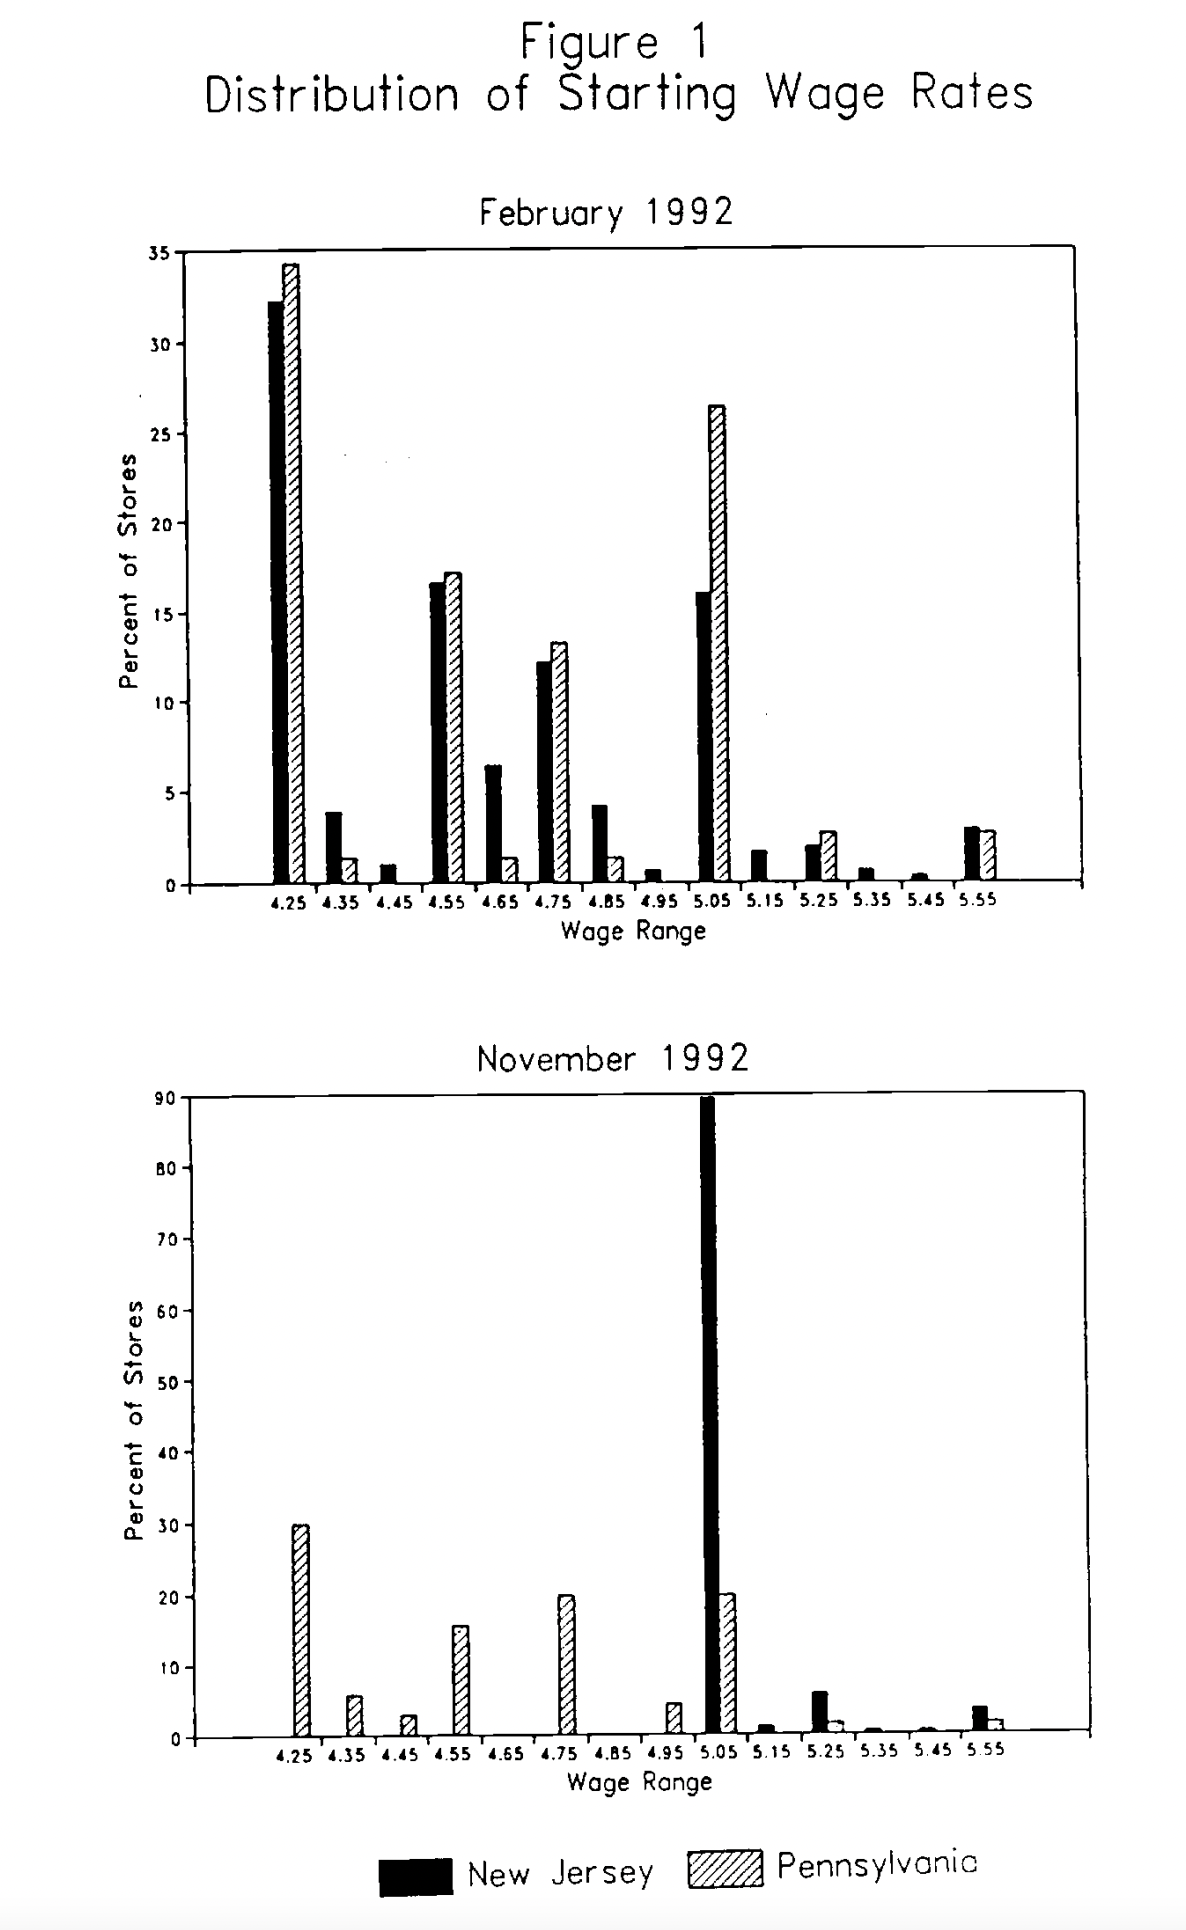
\includegraphics[height = \textheight]{figures/ck_fig1}
\end{frame}

\begin{frame}[t]

\includegraphics<1>[width = \textwidth]{figures/ck_slide1.pdf}
\includegraphics<2>[width = \textwidth]{figures/ck_slide2.pdf}
\includegraphics<3>[width = \textwidth]{figures/ck_slide3.pdf}
\includegraphics<4>[width = \textwidth]{figures/ck_slide4.pdf}
\includegraphics<5>[width = \textwidth]{figures/ck_slide5.pdf}

\end{frame}

\begin{frame}
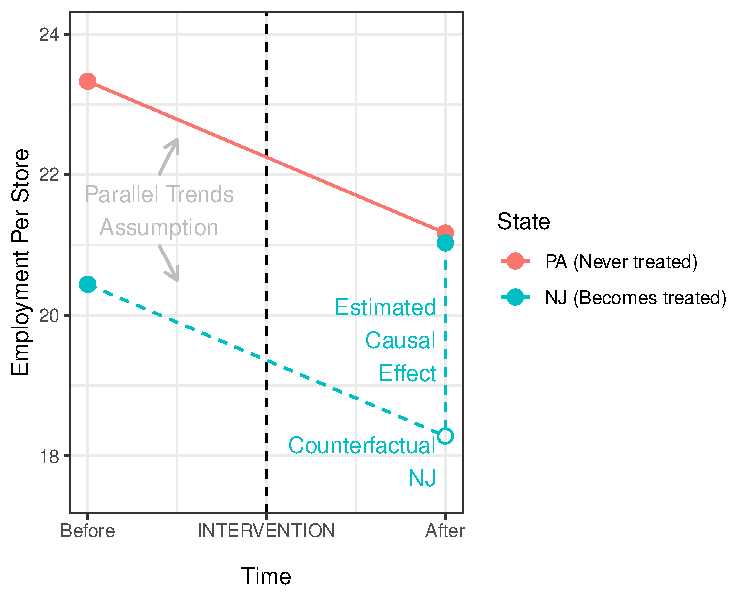
\includegraphics[width = .3\textwidth]{figures/ck_slide5.pdf} \vskip .1in \pause
\bgray{Parallel trends assumption:} \pause If no law had taken effect, then \pause
$$\overbrace{Y_\text{NJ,After}^0  - Y_\text{NJ,Before}^0}^\text{the trend in NJ} \overbrace{=}^\text{would equal} \overbrace{Y_\text{PA,After}^0 - Y_\text{PA,Before}^0}^\text{the trend in PA} $$ \pause
Rearranging yields a formula for the counterfactual outcome \pause
$$
\underbrace{Y_\text{NJ,After}^0}_\text{Counterfactual} \overbrace{=}^\text{By Assumption} \pause \underbrace{Y_\text{NJ,Before}^0 + Y_\text{PA,After}^0 - Y_\text{PA,Before}^0}_\text{Factual}
$$ \pause
$$\text{Effect in NJ} = \underbrace{Y_\text{NJ,After}^1}_\text{Observed}\quad  - \underbrace{Y_\text{NJ,After}^0}_\text{Estimated by Above}$$
\end{frame}

\begin{frame}{Can we test the parallel trends assumption?}

\onslide<2->{\bred{No.}}
\only<1>{$$\overbrace{Y_\text{NJ,After}^0  - Y_\text{NJ,Before}^0}^\text{Assumption: The trend in NJ} \overbrace{=}^\text{would equal} \overbrace{Y_\text{PA,After}^0 - Y_\text{PA,Before}^0}^\text{the trend in PA} $$}
\only<2->{$$\overbrace{\begin{red}\underbrace{Y_\text{NJ,After}^0}_\text{Not Observable}\end{red}  - Y_\text{NJ,Before}^0}^\text{Assumption: The trend in NJ} \overbrace{=}^\text{would equal} \overbrace{Y_\text{PA,After}^0 - Y_\text{PA,Before}^0}^\text{the trend in PA} $$} \vskip .2in
\onslide<3->{You can make it credible by looking at many pre-treatment periods}

\end{frame}

\begin{frame}[t]{DID would be very credible}
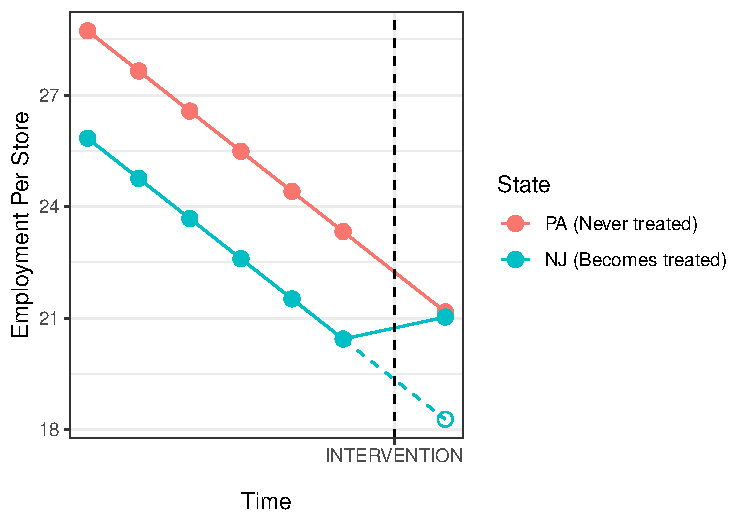
\includegraphics[width = \textwidth]{figures/parallel_trends_credible.pdf}
\end{frame}

\begin{frame}[t]{DID would be very doubtful}
\includegraphics<1>[width = \textwidth]{figures/parallel_trends_doubtful.pdf}
\includegraphics<2>[width = \textwidth]{figures/parallel_trends_doubtful_2.pdf}
\includegraphics<3>[width = \textwidth]{figures/parallel_trends_doubtful_3.pdf}
\end{frame}

\begin{frame}[t]{Interrupted time series\footnote{Bernal, J. L., Cummins, S., \& Gasparrini, A. (2017). \bref{https://doi.org/10.1093/ije/dyw098}{Interrupted time series regression for the evaluation of public health interventions: A tutorial.} International Journal of Epidemiology, 46(1), 348-355.}} \pause \vskip .2in
You study one unit. It is untreated. Then it is treated. \vskip .2in
\begin{center}
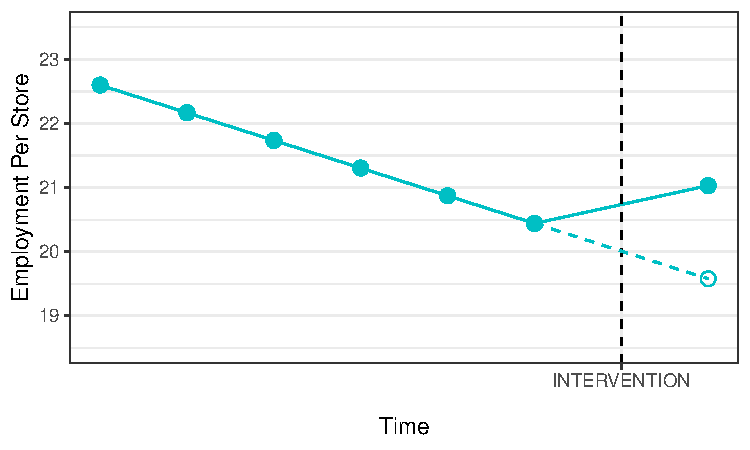
\includegraphics[width = .4\textwidth]{figures/parallel_trends_doubtful_4.pdf} \vskip .1in
\end{center}
\only<3-5>{In what settings does this work well?
\begin{itemize}
\item<4-5> When you have a strong pre-treatment trend to forecast $Y^0_t$
\item<5> When you don't have a comparable unit that is never treated
\end{itemize}
}
\only<6>{\bgray{Theoretical Estimand}\\$$\E(Y^1 - Y^0\mid T > t_\text{Intervention})$$}
\only<7-8>{\bgray{Identifying Assumption}
\begin{itemize}
\item<8> In the absence of the intervention,\\the pre-intervention trend in $Y^0$ would have continued
\end{itemize}}
\only<9->{Concrete steps:}
\begin{enumerate}
\item<10-> Learn a model on the pre-treatment period
\begin{itemize}
\item<11-> Evaluation metric: Forecast within the pre-treatment period
\end{itemize}
\item<12-> Forecast $Y^0$ for the post-treatment period
\end{enumerate}
\end{frame}

\begin{frame}[t]{Interrupted time series: When it becomes doubtful}
\includegraphics<2>[width = \textwidth]{figures/its_problem_1}
\includegraphics<3>[width = \textwidth]{figures/its_problem_2}
\includegraphics<4>[width = \textwidth]{figures/its_problem_3}
\includegraphics<5>[width = \textwidth]{figures/its_problem_4}
\includegraphics<6>[width = \textwidth]{figures/its_problem_5}
\end{frame}

\begin{frame}{Interrupted time series: Recap}
\begin{itemize}
\item ITS applies when treatment turns on at one time for all units
\item ITS requires a parametric model to extrapolate
\item ITS is most credible near the time when treatment turns on
\end{itemize}
\end{frame}

\begin{frame}{When to use each method}
\begin{itemize}\setlength\itemsep{.5em}\small
\item Difference in difference
\begin{itemize}\setlength\itemsep{.1em}\footnotesize
\item One unit becomes treated \hfill New Jersey
\item One unit never becomes treated \hfill Pennsylvania
\item The trends in $Y^0$ are parallel
\end{itemize}
\item Interrupted time series
\begin{itemize}\setlength\itemsep{.1em}\footnotesize
\item Everyone becomes treated at $X = c$\hfill New drug
\item You believe you can forecast $Y^0$\hfill Deaths would\\from $X < c$ to $X > c$\hfill have been stable
\end{itemize}
\end{itemize}
\end{frame}

\begin{frame}{Regression discontinuity\footnote{Cattaneo, M. D., \& Titiunik, R. (2022). \bref{https://doi.org/10.1146/annurev-economics-051520-021409}{Regression discontinuity designs.} Annual Review of Economics, 14, 821-851.}}
\begin{tikzpicture}[x = \textwidth, y = .8\textheight]
\node at (0,0) {};
\node at (1,1) {};
\node<2->[anchor = west] (fig) at (0,.5) {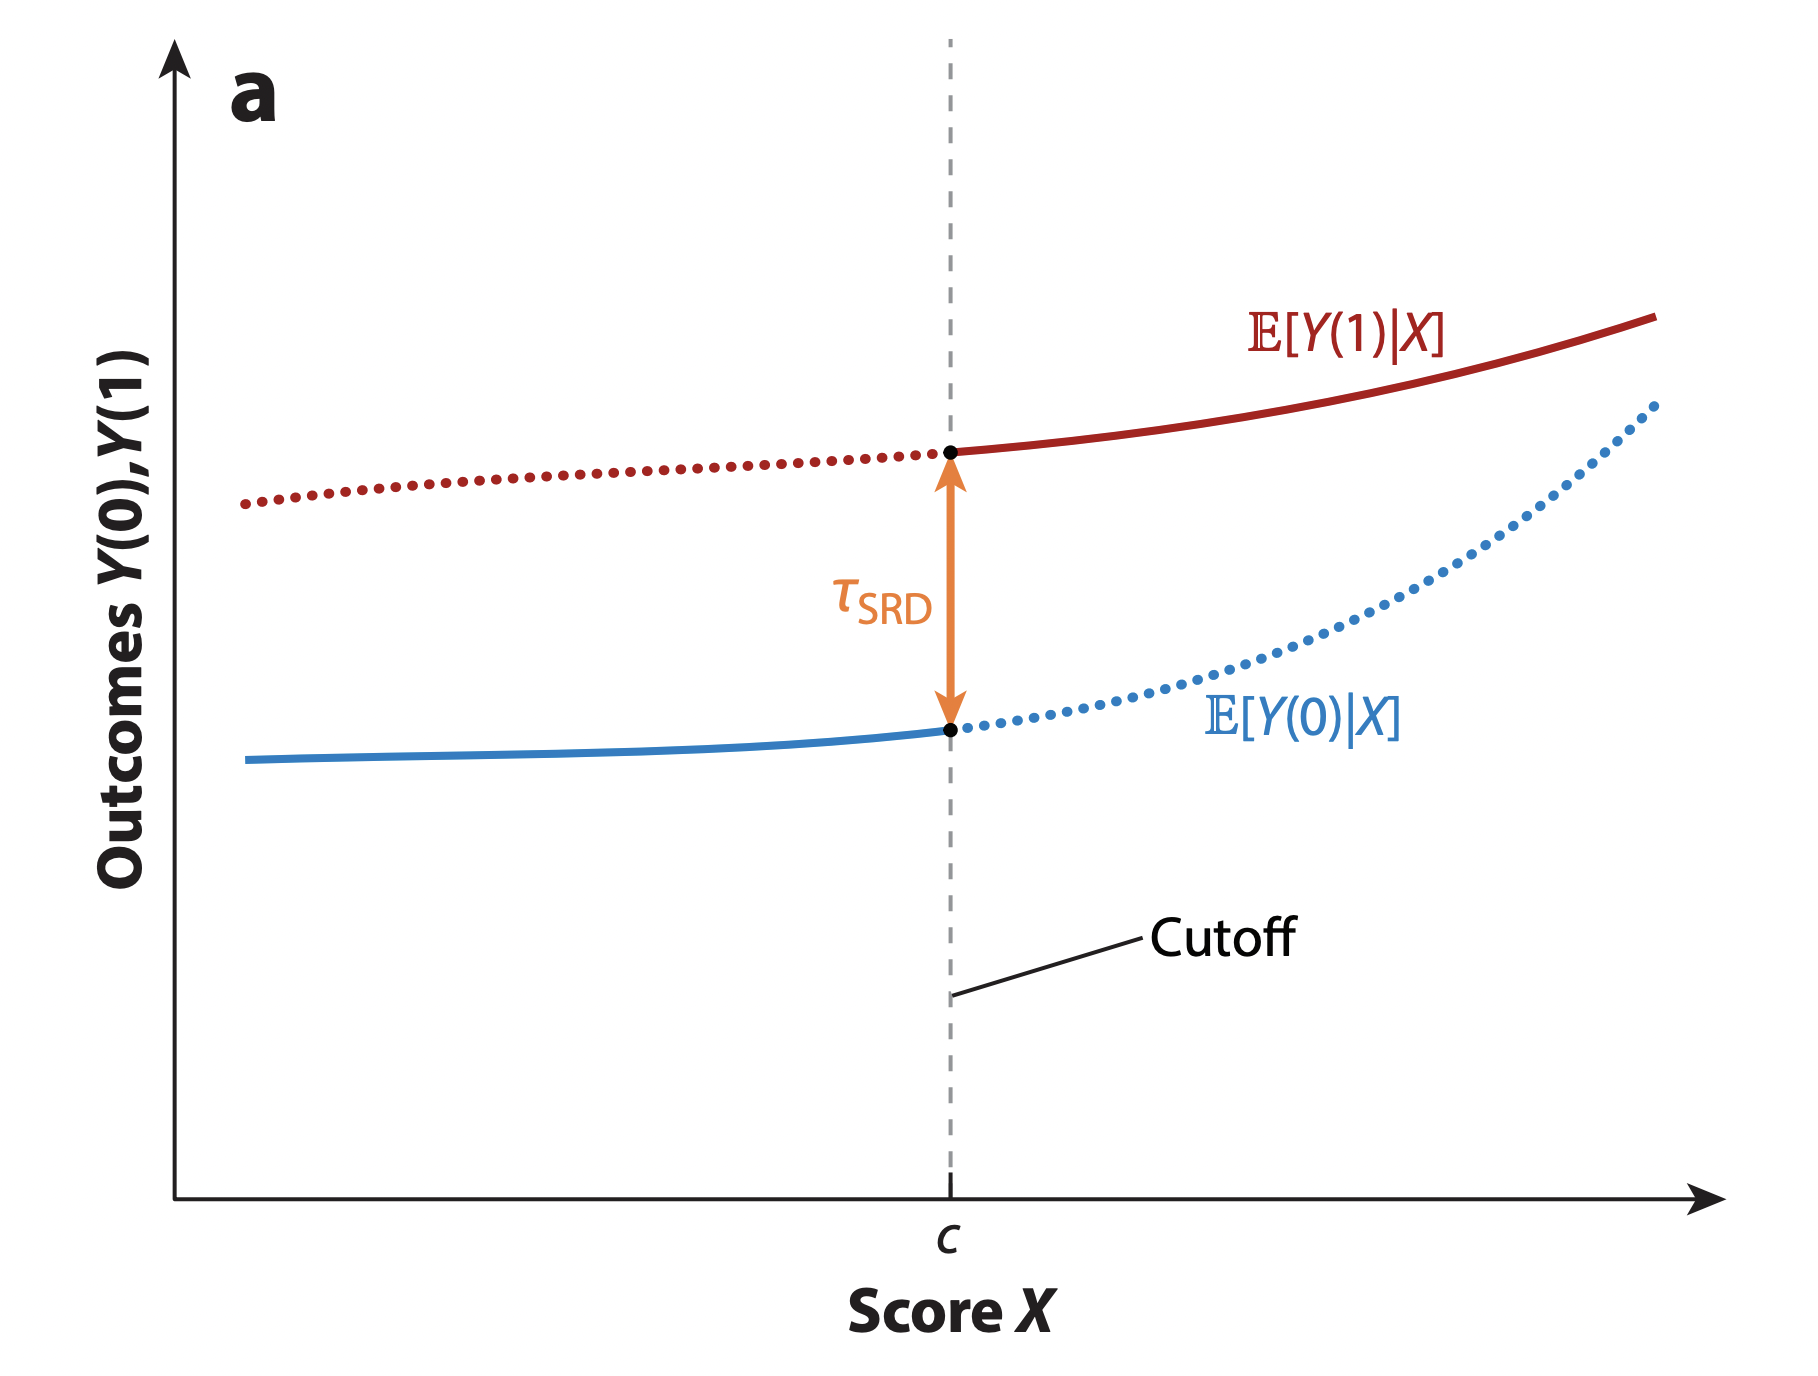
\includegraphics[width = .5\textwidth]{figures/ct_fig1a}};
\node<2->[anchor = south west, font = {\footnotesize\bf}] at (fig.north west) {Cattaneo \& Titiunik 2022 Fig 1a};
\node<3-6>[anchor = north west] at (.6, .9) {\bgray{Examples}};
\node<4-6>[anchor = north west, align = left, font = \small] at (.6, .8) {$X$ is PSAT test score\\$c$ is a score cutoff\\$A$ is National Merit Scholarship\\\begin{tiny}(\href{https://osf.io/tc5j7/download}{Thistlewaite \& Campbell 1960})\end{tiny}};
\node<5-6>[anchor = north west, align = left, font = \small] at (.6, .55) {$X$ is vote share\\$c$ is 50\%\\$A$ is winning the election\\\begin{tiny}(\href{https://imai.fas.harvard.edu/research/files/RD.pdf}{De la Cuesta \& Imai 2016})\end{tiny}};
\node<6>[anchor = north west, align = left, font = \small] at (.6, .3) {$X$ is date\\$c$ is 2am Nov 6 2022\\$A$ is hours of PM darkness};
\node<8-10>[anchor = north west, align = left] at (.6,.9) {\bgray{Theoretical Estimand}\\$\E(Y(1) - Y(0) \mid X = c)$};
\node<9-10>[anchor = north west, align = left] at (.6,.7) {\bgray{Empirical Estimand}\\$\text{lim}_{x\downarrow c}\E(Y\mid X = x)$\\\phantom{empirical}$-$\\$\text{lim}_{x\uparrow c}\E(Y\mid X = x)$};
\node<10>[anchor = north west, align = left] at (.6,.4) {\bgray{Identifying Assumptions}\\$\E(Y(1) \mid X = x)$ and\\$\E(Y(0) \mid X = x)$ are\\continuous at $x = c$\\{}\\and $f_X(x) > 0$ for $x$ near $c$};
\node<12->[anchor = north west, align = left] (p) at (.6,.85) {\bgray{Promises of RD}};
\node<13->[anchor = north west, align = left] (p1) at (p.south west) {--- Highly credible};
\node<14->[anchor = north west, align = left] (p2) at (p1.south west) {--- Easy to visualize};
\node<12->[anchor = north west, align = left] (d) at (.6,.5) {\bgray{Drawbacks of RD}};
\node<15->[anchor = north west, align = left] (d1) at (d.south west) {--- Local to $X = c$};
\node<16->[anchor = north west, align = left] (d2) at (d1.south west) {--- Sensitive to sorting};
\node<17->[anchor = north east, align = right] at (d2.south east) {(people moving\\strategically over\\the cutoff)};
\end{tikzpicture}
\end{frame}

\begin{frame}{When to use each method}
\begin{itemize}\setlength\itemsep{.5em}\small
\item Difference in difference
\begin{itemize}\setlength\itemsep{.1em}\footnotesize
\item One unit becomes treated \hfill New Jersey
\item One unit never becomes treated \hfill Pennsylvania
\item The trends in $Y^0$ are parallel
\end{itemize}
\item Interrupted time series
\begin{itemize}\setlength\itemsep{.1em}\footnotesize
\item Everyone becomes treated at $X = c$\hfill New drug
\item You believe you can forecast $Y^0$\hfill Deaths would\\from $X < c$ to $X > c$\hfill have been stable
\end{itemize}
\item Regression discontinuity
\begin{itemize}\setlength\itemsep{.1em}\footnotesize
\item Everyone becomes treated at $X = c$ \hfill Win the election
\item You want a local estimate\\$\E(Y^1 - Y^0 \mid X = c)$ at the cutoff\hfill Close elections
\item $Y^0$ and $Y^1$ are continuous at $X = c$
\end{itemize}
\end{itemize}
\end{frame}

\begin{frame}{Synthetic control\footnote{Abadie, A., Diamond, A., \& Hainmueller, J. (2010). \bref{http://www.jenshainmueller.de/Paper/ccs.pdf}{Synthetic control methods for comparative case studies: Estimating the effect of California’s tobacco control program.} Journal of the American Statistical Association, 105(490), 493-505.}} \pause
In 1988, California implemented a tobacco control program \pause
\begin{itemize}
\item New tax: 25 cents per pack \pause
\item Money earmarked for smoking-reduction programs
\end{itemize} \vskip .2in \pause
How much did it reduce CA cigarette sales in 1990? 1995? 2000?
\end{frame}

\begin{frame}{Synthetic control\footnote{Abadie, A., Diamond, A., \& Hainmueller, J. (2010). \bref{http://www.jenshainmueller.de/Paper/ccs.pdf}{Synthetic control methods for comparative case studies: Estimating the effect of California’s tobacco control program.} Journal of the American Statistical Association, 105(490), 493-505.}}

\begin{tikzpicture}[x = \textwidth, y = .6\textheight]
\node at (0,0) {};
\node at (1,1) {};
\node[anchor = west] at (0,.5) {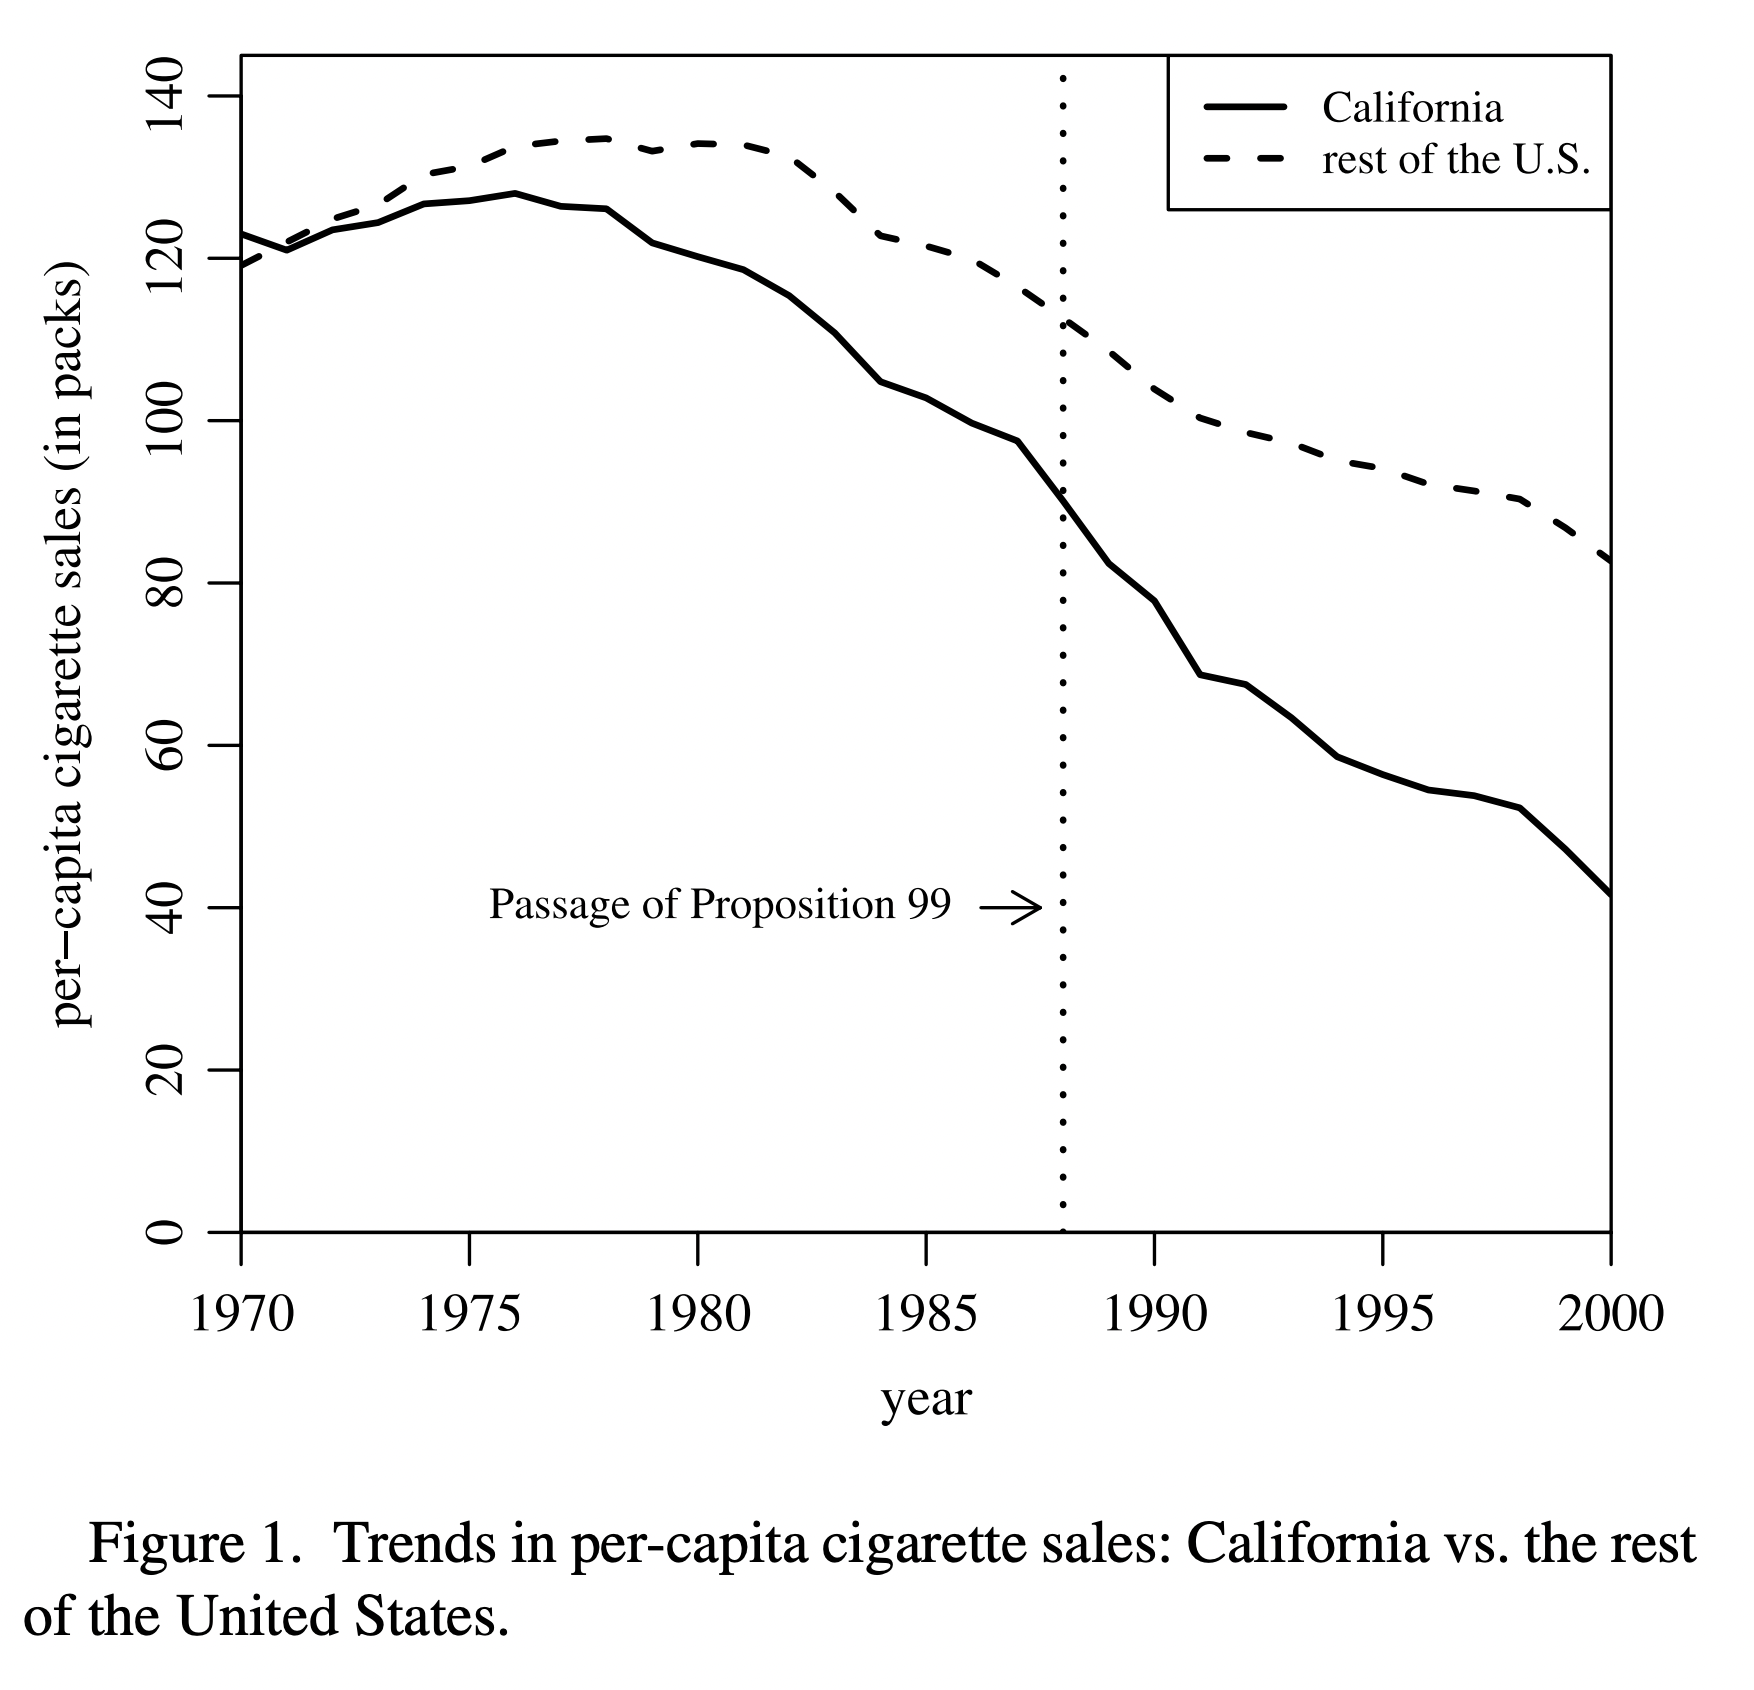
\includegraphics[height = .6\textheight]{figures/synth_fig1}};
\node[anchor = north west] at (.55,1) {Can't use RD};
\node[anchor = north west, font = \small] at (.55,.92) {--- Effect at 1988 not of interest};
\node[anchor = north west] at (.55,.8) {Can't use ITS};
\node[anchor = north west, font = \small] at (.55,.72) {--- Hard to extrapolate $Y^0$ trend};
\node[anchor = north west] at (.55,.6) {Can't use DID};
\node[anchor = north west, font = \small] at (.55,.52) {--- No other state like CA};
\node[anchor = north west, align = left] (idea) at (.65,.35) {Idea: Create a\\\bblue{synthetic CA}\\to estimate\\$Y^0_\text{CA,t}$ for $t \geq 1988$};
\draw[gray, thick] (idea.north east) -- (idea.north west) -- (idea.south west) -- (idea.south east);
\end{tikzpicture}

\end{frame}

\begin{frame}{Synthetic control\footnote{Abadie, A., Diamond, A., \& Hainmueller, J. (2010). \bref{http://www.jenshainmueller.de/Paper/ccs.pdf}{Synthetic control methods for comparative case studies: Estimating the effect of California’s tobacco control program.} Journal of the American Statistical Association, 105(490), 493-505.}}{Synthetic CA as a weighted average of other states}

\begin{center}
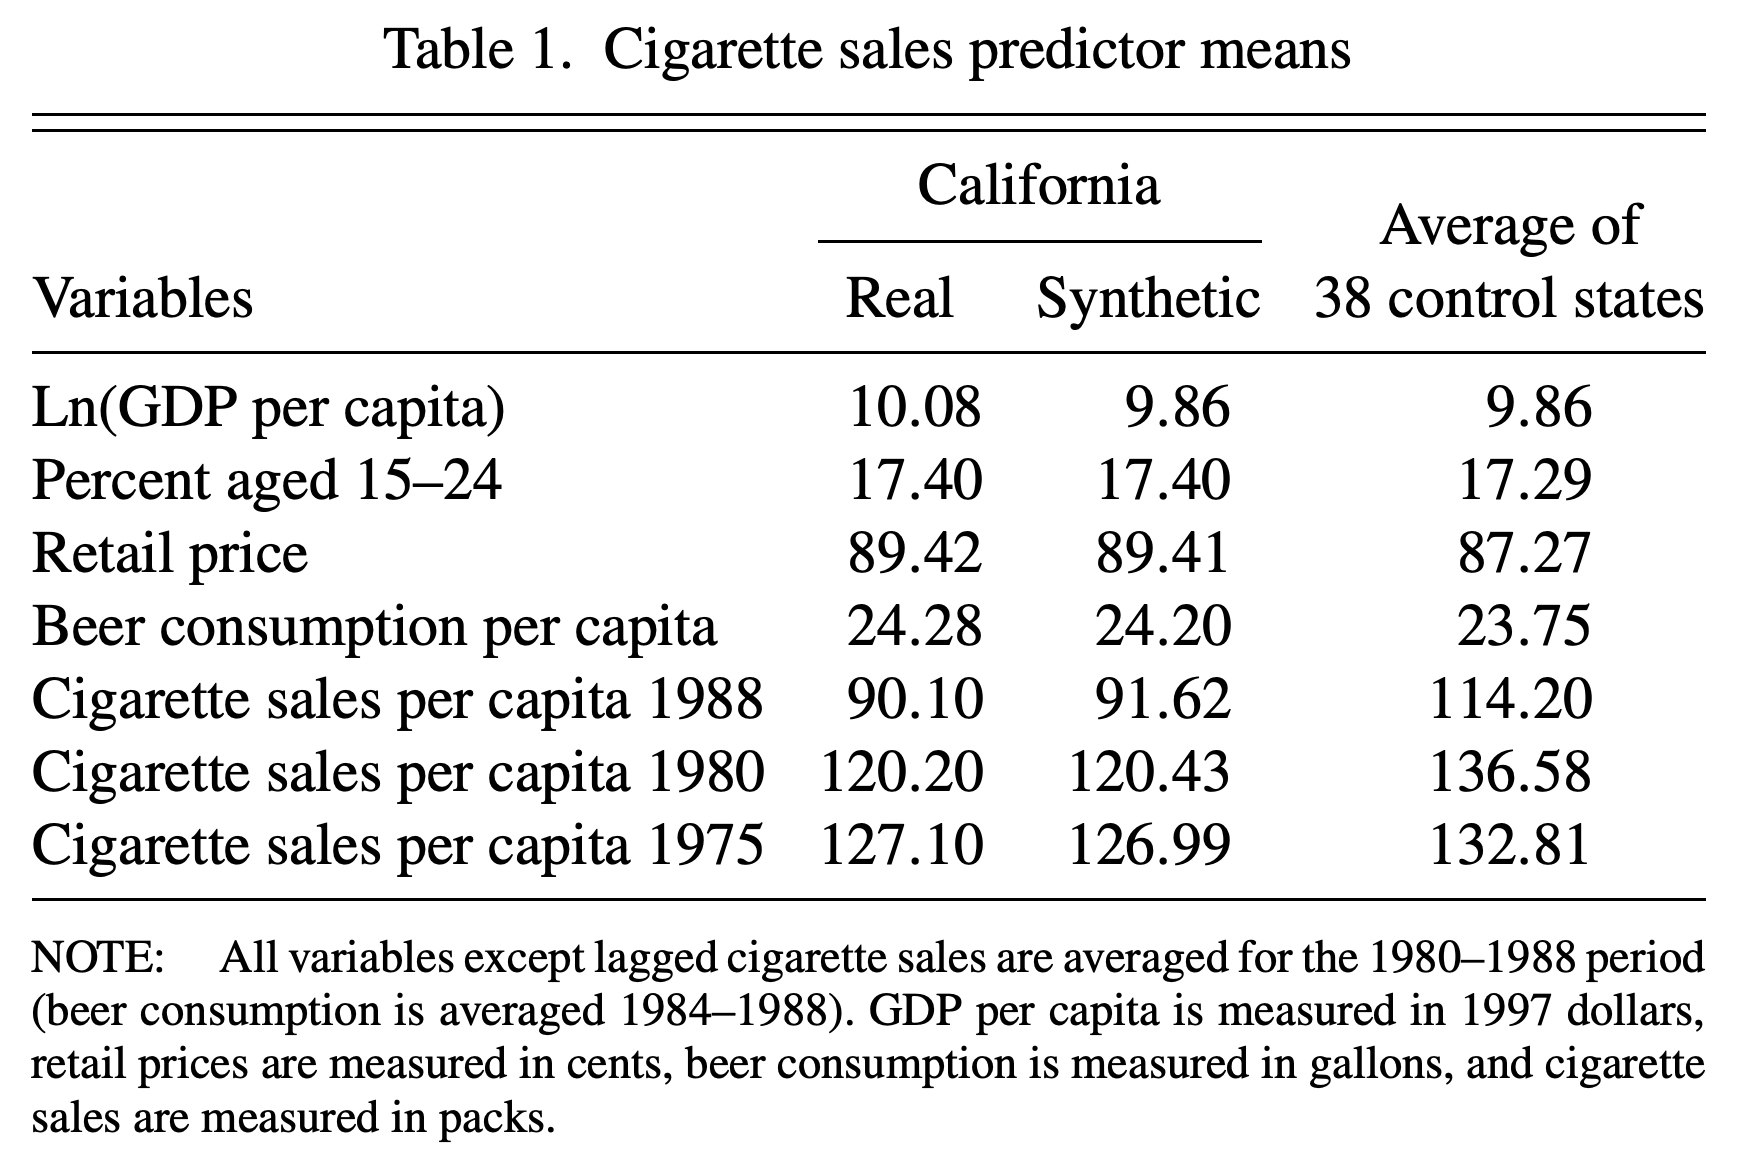
\includegraphics[height = .5\textheight]{figures/synth_tab1} \vskip .1in
\end{center}

\end{frame}

\begin{frame}{Synthetic control\footnote{Abadie, A., Diamond, A., \& Hainmueller, J. (2010). \bref{http://www.jenshainmueller.de/Paper/ccs.pdf}{Synthetic control methods for comparative case studies: Estimating the effect of California’s tobacco control program.} Journal of the American Statistical Association, 105(490), 493-505.}}{Synthetic CA as a weighted average of other states}

\begin{tabular}{rll}
Theoretical Estimand: & $\tau(t) = Y^1_{\text{CA},t}-Y^0_{\text{CA},t}$ & $t \geq 1988$ \\ \pause
\\
Empirical Estimand: & $\theta(t) = Y^1_{\text{CA},t}-Y^0_{\text{SyntheticCA},t}$ & $t \geq 1988$ \\ \pause
\\
Identifying Assumption: & $\underbrace{Y^0_{\text{CA},t}}_\text{Counterfactual} = \quad\underbrace{Y^0_{\text{SyntheticCA},t}}_\text{Factual}$ & $t \geq 1988$
\end{tabular}

\end{frame}

\begin{frame}{Synthetic control\footnote{Abadie, A., Diamond, A., \& Hainmueller, J. (2010). \bref{http://www.jenshainmueller.de/Paper/ccs.pdf}{Synthetic control methods for comparative case studies: Estimating the effect of California’s tobacco control program.} Journal of the American Statistical Association, 105(490), 493-505.}}

\centering
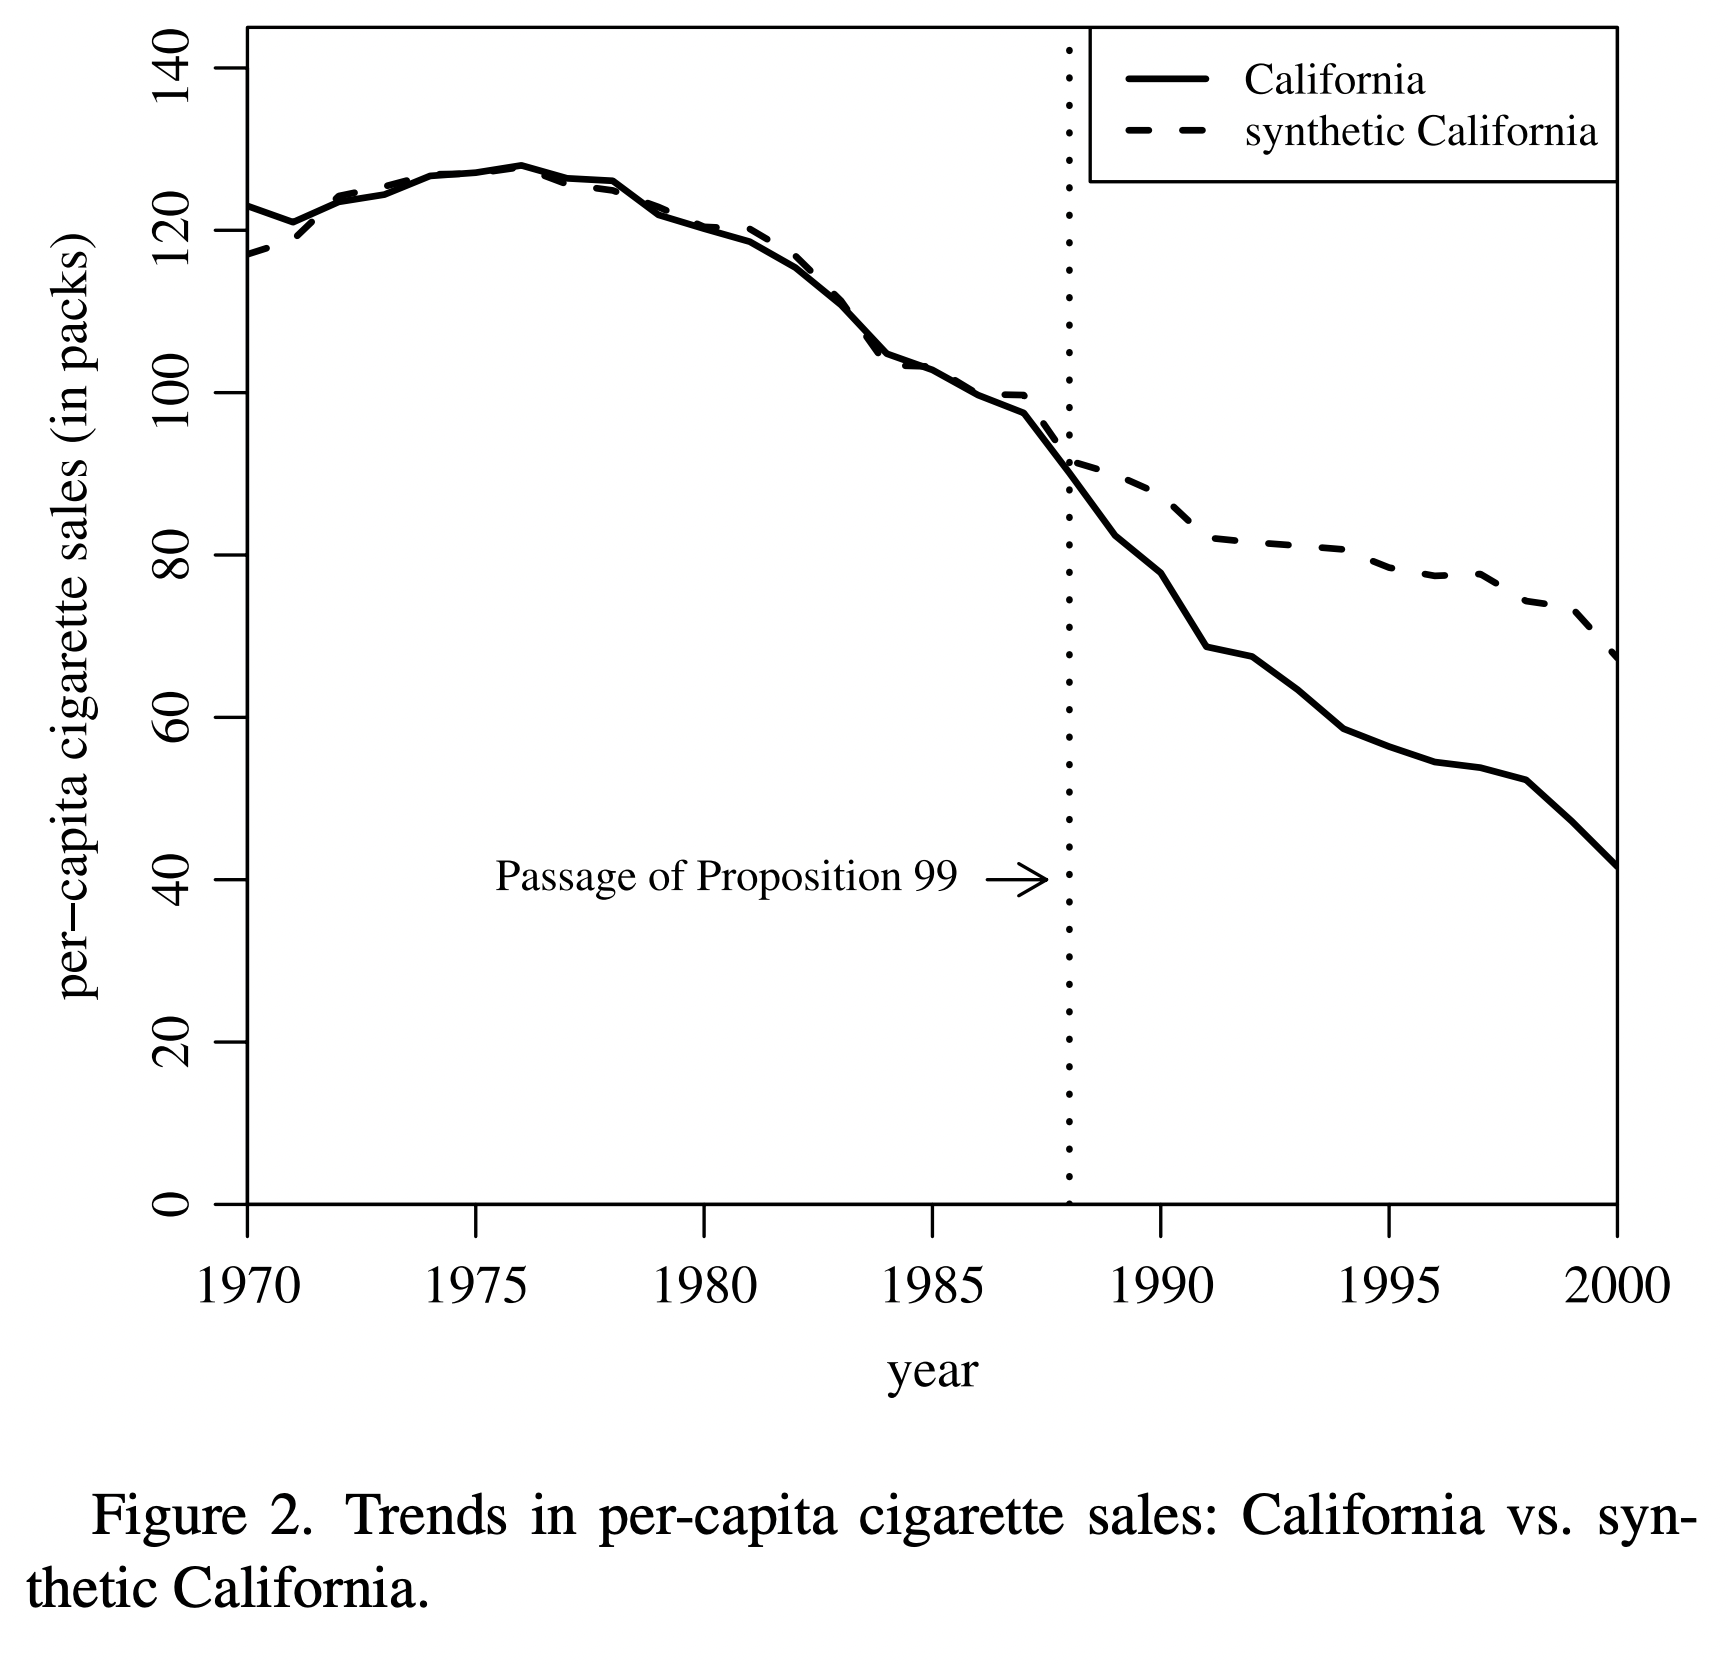
\includegraphics[height = .6\textheight]{figures/synth_fig2}

\end{frame}

\begin{frame}{When to use each method}
\begin{itemize}\setlength\itemsep{.5em}\small
\item Difference in difference
\begin{itemize}\setlength\itemsep{.1em}\footnotesize
\item One unit becomes treated \hfill New Jersey
\item One unit never becomes treated \hfill Pennsylvania
\item The trends in $Y^0$ are parallel
\end{itemize}
\item Interrupted time series
\begin{itemize}\setlength\itemsep{.1em}\footnotesize
\item Everyone becomes treated at $X = c$\hfill New drug
\item You believe you can forecast $Y^0$\hfill Deaths would\\from $X < c$ to $X > c$\hfill have been stable
\end{itemize}
\item Regression discontinuity
\begin{itemize}\setlength\itemsep{.1em}\footnotesize
\item Everyone becomes treated at $X = c$ \hfill Win the election
\item You want a local estimate\\$\E(Y^1 - Y^0 \mid X = c)$ at the cutoff\hfill Close elections
\item $Y^0$ and $Y^1$ are continuous at $X = c$
\end{itemize}
\item Synthetic control
\begin{itemize}\setlength\itemsep{.1em}\footnotesize
\item One unit becomes treated \hfill California
\item Many units are never treated \hfill Other states
\item You want to extrapolate far from the cutoff \hfill 1988$\rightarrow$2000
\end{itemize}
\end{itemize}
\end{frame}

\goalsframe


\begin{frame}{Let me know what you are thinking}

\begin{huge} \bref{https://tinyurl.com/CausalQuestions}{tinyurl.com/CausalQuestions} \end{huge}
\vskip .7in

Office hours TTh 11am-12pm and at \bref{https://calendly.com/ianlundberg/office-hours}{calendly.com/ianlundberg/office-hours}\\Come say hi!

\end{frame}


\end{document}
